\section{数据描述与预处理}

\subsection{数据来源与文件清单}

题目提供两大数据集：一是"无人机应急物资运输基础数据"（5 个 Excel 文件），给出调度中心、服务区、货箱需求、机型装备与通信链路的全部参数；二是"镇龙乡地理空间数据"，给出 30\,m 数字高程模型（DEM）及村镇点位、水体、水系、道路等要素。本文计算口径以附件数据为准，空间坐标与公开地理数据仅用于描述测试场景。数据文件清单与用途见表~\ref{tab:data_files}。

\begin{table}[htbp]
\centering
\caption{数据文件清单与用途}
\label{tab:data_files}
\small
\begin{tabular}{ll}
\toprule
\textbf{数据文件} & \textbf{主要内容与用途} \\
\midrule
调度中心与服务区.xlsx & O01 及 S001--S015 的经纬度与海拔，节点坐标 \\
物资需求与配送时限.xlsx & 各服务区物资需求、货箱属性（质量/体积）、期望送达时间、应急优先系数、逐箱清单 \\
运输无人机数据.xlsx & A/B/C 机型空载/满载航程、最大载货质量、装载体积、速度、电池可用能量与返航余量 \\
中继无人机数据.xlsx & 中继机巡航/爬升/下降/悬停功率、能源组件参数、准备/建链时间 \\
通信链路参数.xlsx & 固定网关 G01、运输机、中继机的发射功率、天线增益、接收灵敏度、衰落裕量、系统损耗 \\
镇龙乡地理空间数据 & 30\,m DEM、村镇点位、水体、水系、道路（用于地形净空与通信遮挡判定） \\
\bottomrule
\end{tabular}
\end{table}

\subsection{物资需求与应急优先级}

各服务区物资以饮用水、应急食品为主，兼有医疗物资与首批保障箱，配送时限呈明显分层。图~\ref{fig:data_priority} 给出各服务区应急优先系数的热力图，可见医疗物资与首批保障货箱的应急优先系数显著高于普通饮用水与生活物资，这一差异直接进入问题二、三的配送及时性目标 $f_1$ 与硬时限约束，是资源调度中"紧迫优先"规则的依据。

\begin{figure}[htbp]
\centering
\subfloat[应急优先系数热力图]{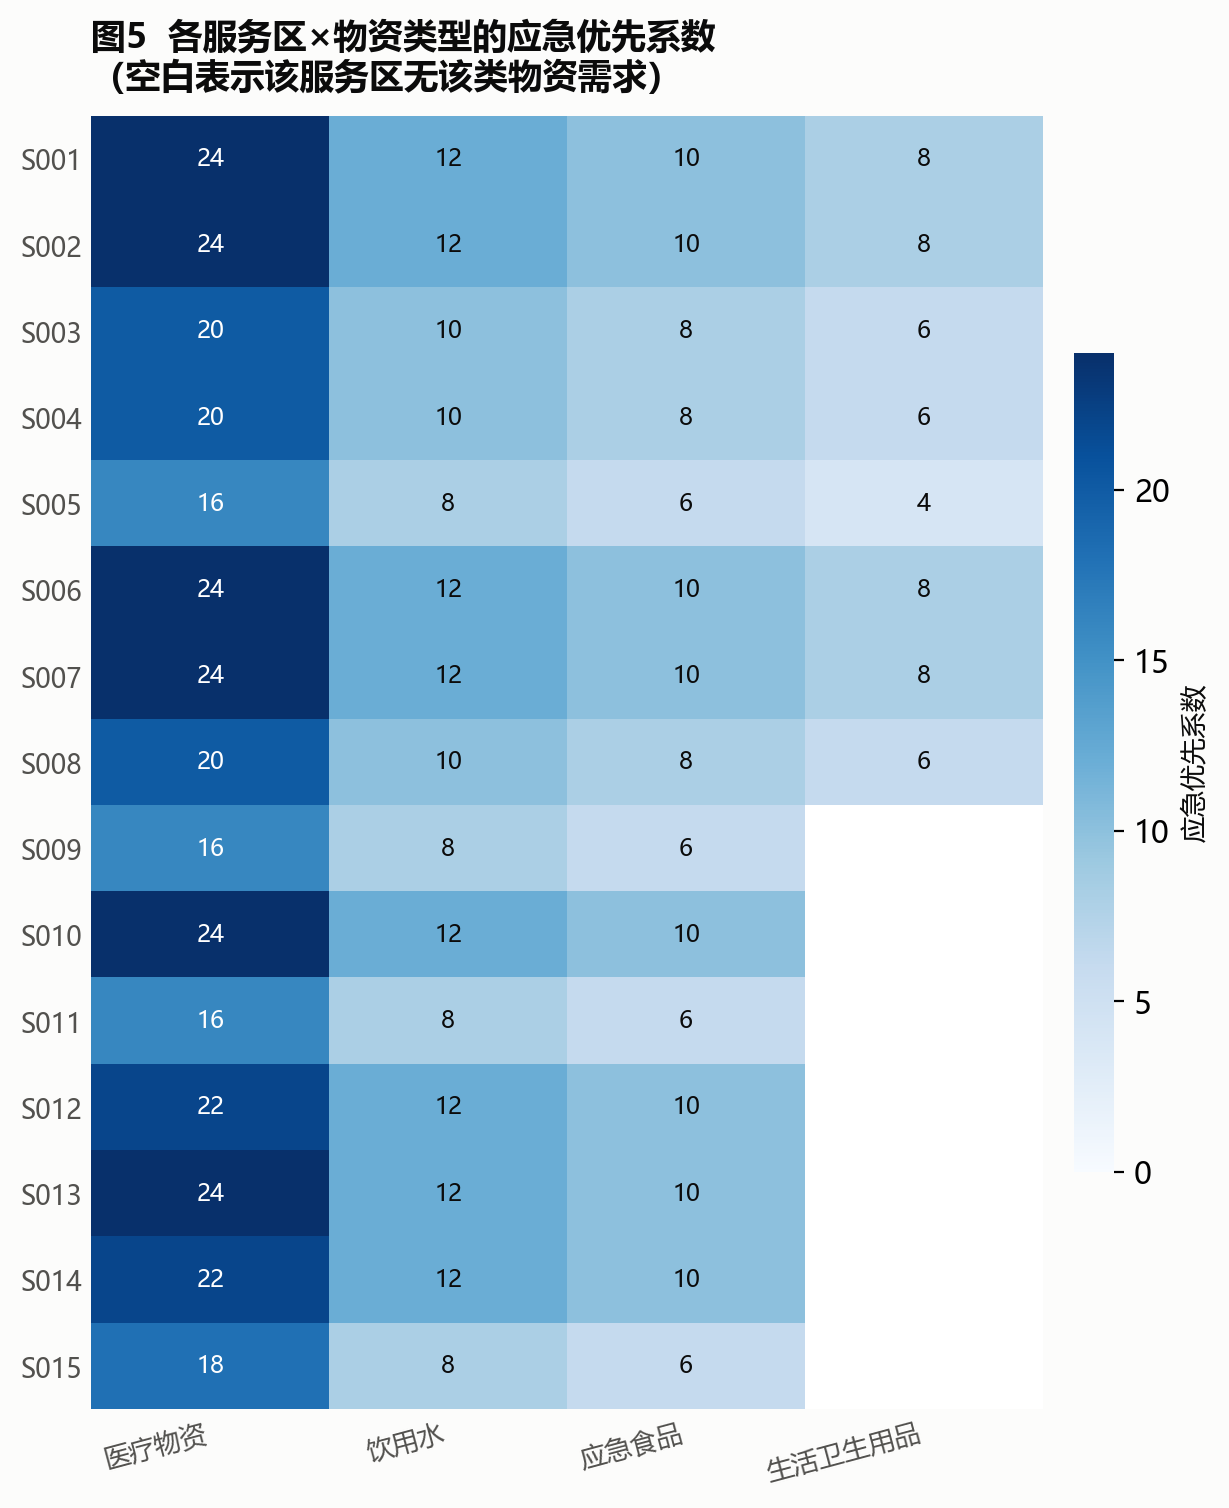
\includegraphics[width=0.48\textwidth]{figures/05_应急优先系数热力图.png}\label{fig:data_priority}}
\hfill
\subfloat[逐箱货箱特征分布]{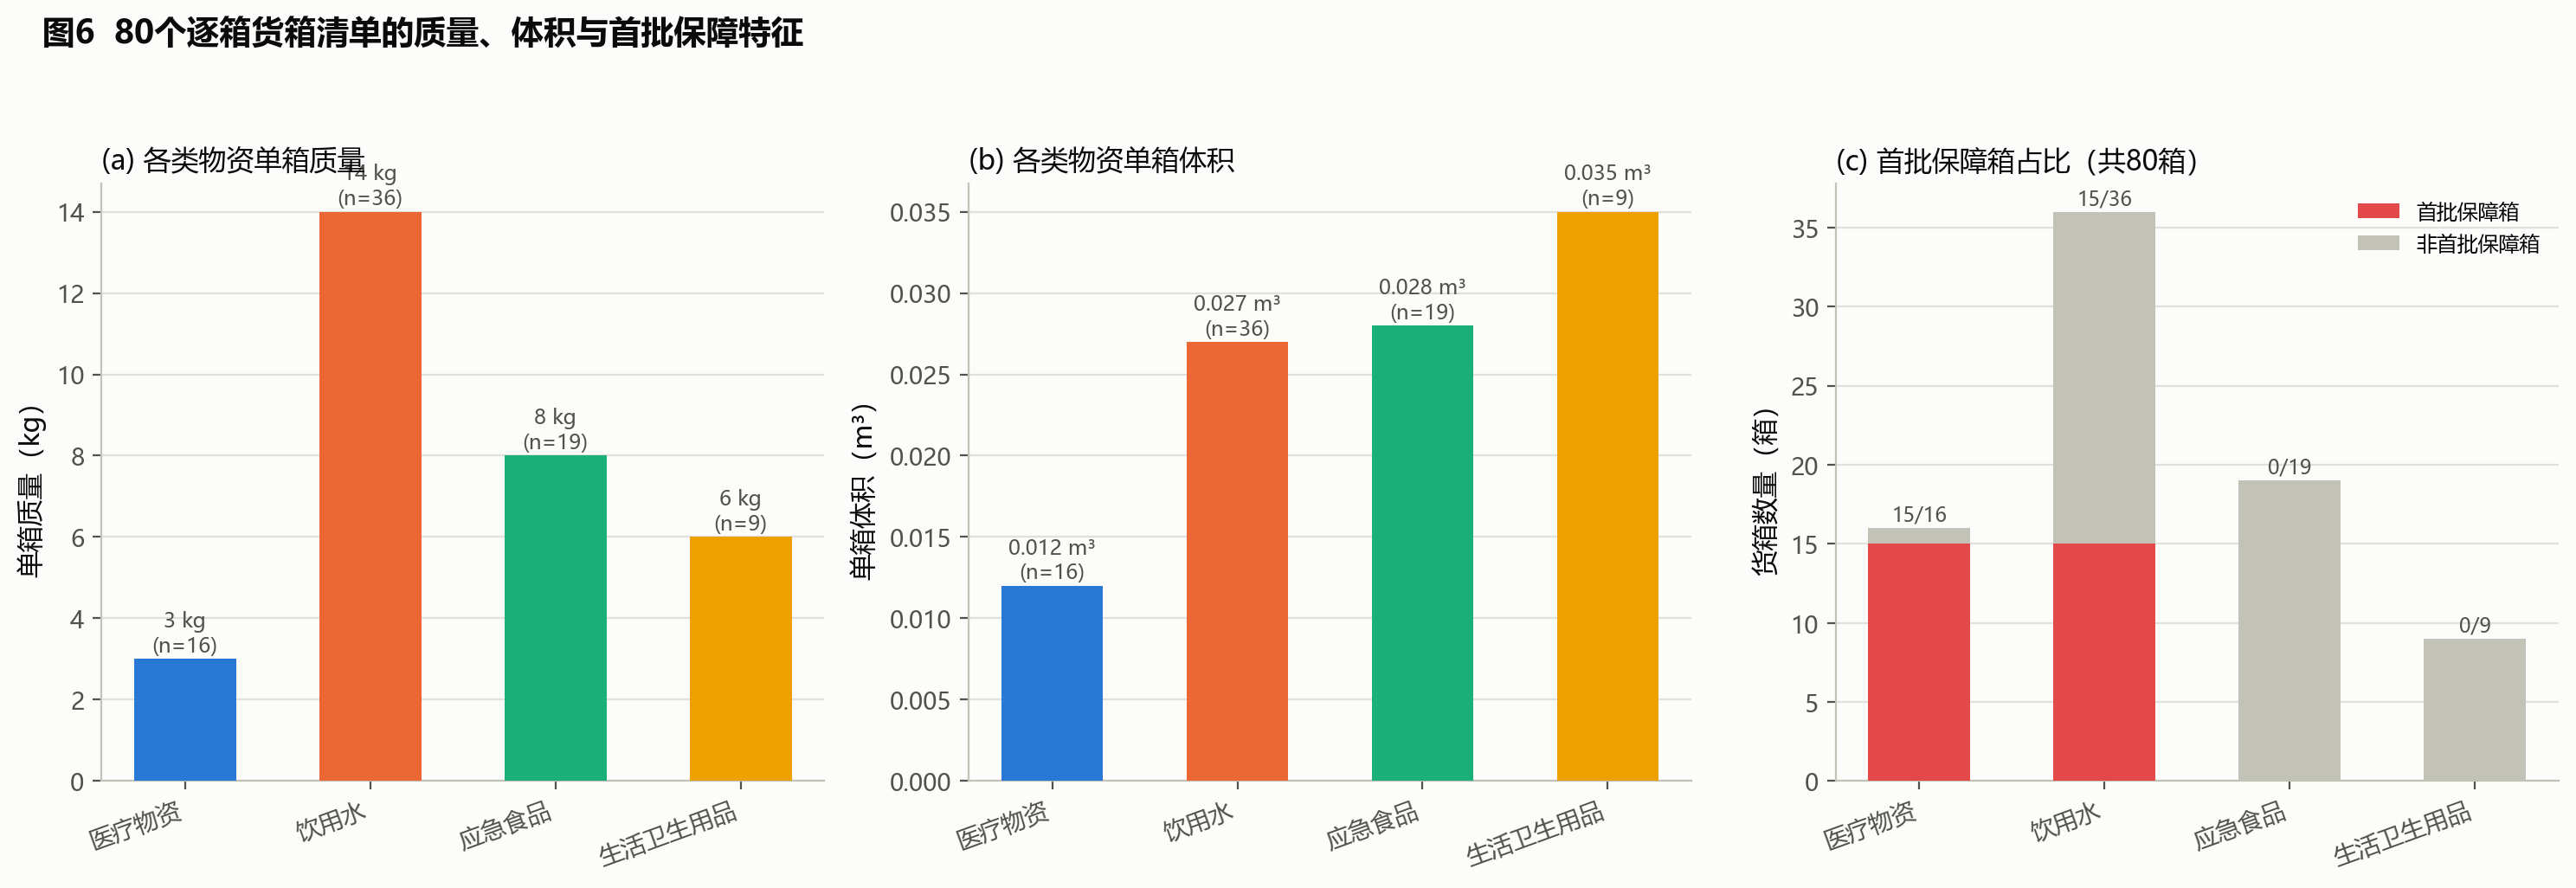
\includegraphics[width=0.48\textwidth]{figures/06_逐箱货箱特征分布.png}\label{fig:data_box}}
\caption{应急优先系数与逐箱货箱特征}
\label{fig:data_demand}
\end{figure}

图~\ref{fig:data_box} 给出 80 个货箱的质量与体积分布，可见货箱质量集中于数千克至十余千克、体积集中于 $0.02$--$0.05$\,m$^3$ 区间，单箱质量/体积均不超过任一机型上限，为问题一"单箱必可被某机型单独运输"的可行性前提提供了数据支撑。

\subsection{运输无人机与共享电池参数}

题目配置 A/B/C 三种运输无人机机型共 8 架实体机（A 型 4、B 型 2、C 型 2），并配共享电池组（A 型 6、B 型 4、C 型 4 组）。图~\ref{fig:data_drone} 给出三种机型的参数对比，可见机型 C 的载货质量与装载体积最大、机型 A 最小，而空载/满载标准航程与电池可用能量亦随机型递增；图~\ref{fig:data_battery} 给出共享电池库存与完全充电时间。机队规模与电池数量共同构成问题二、三的资源瓶颈约束。

\begin{figure}[htbp]
\centering
\subfloat[机型参数对比]{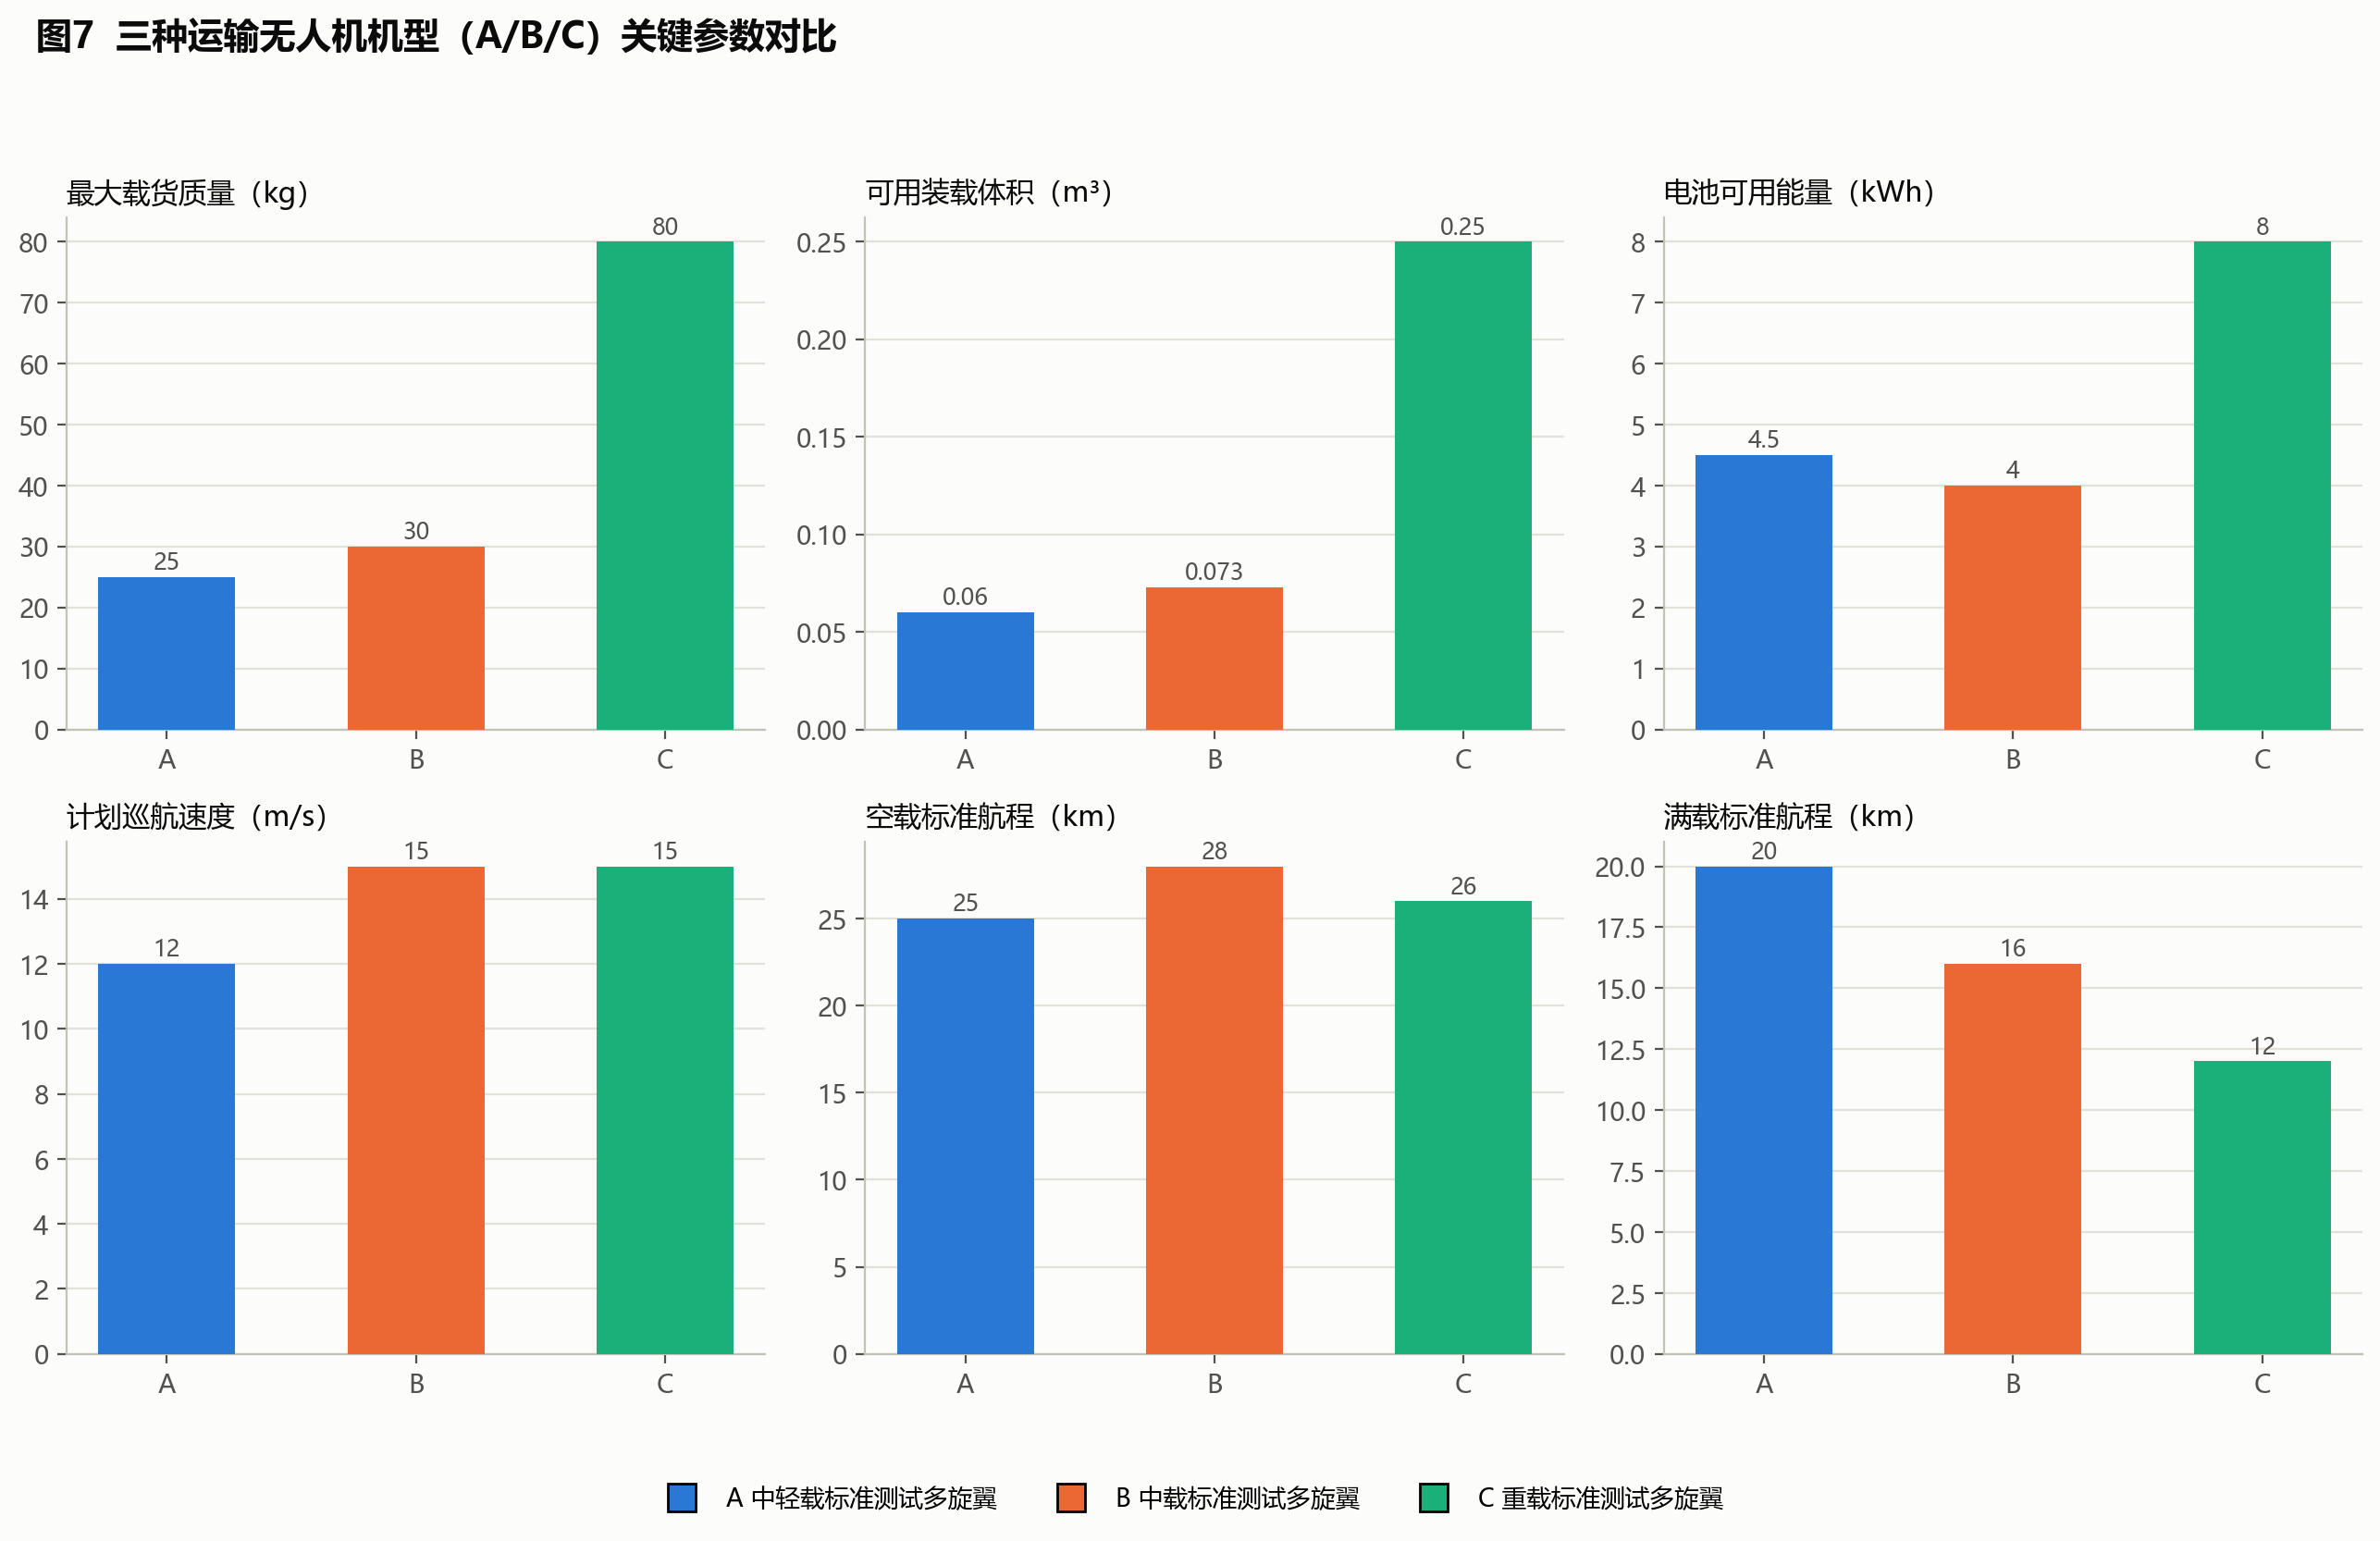
\includegraphics[width=0.48\textwidth]{figures/07_运输无人机机型参数对比.png}\label{fig:data_drone}}
\hfill
\subfloat[共享电池库存与充电时间]{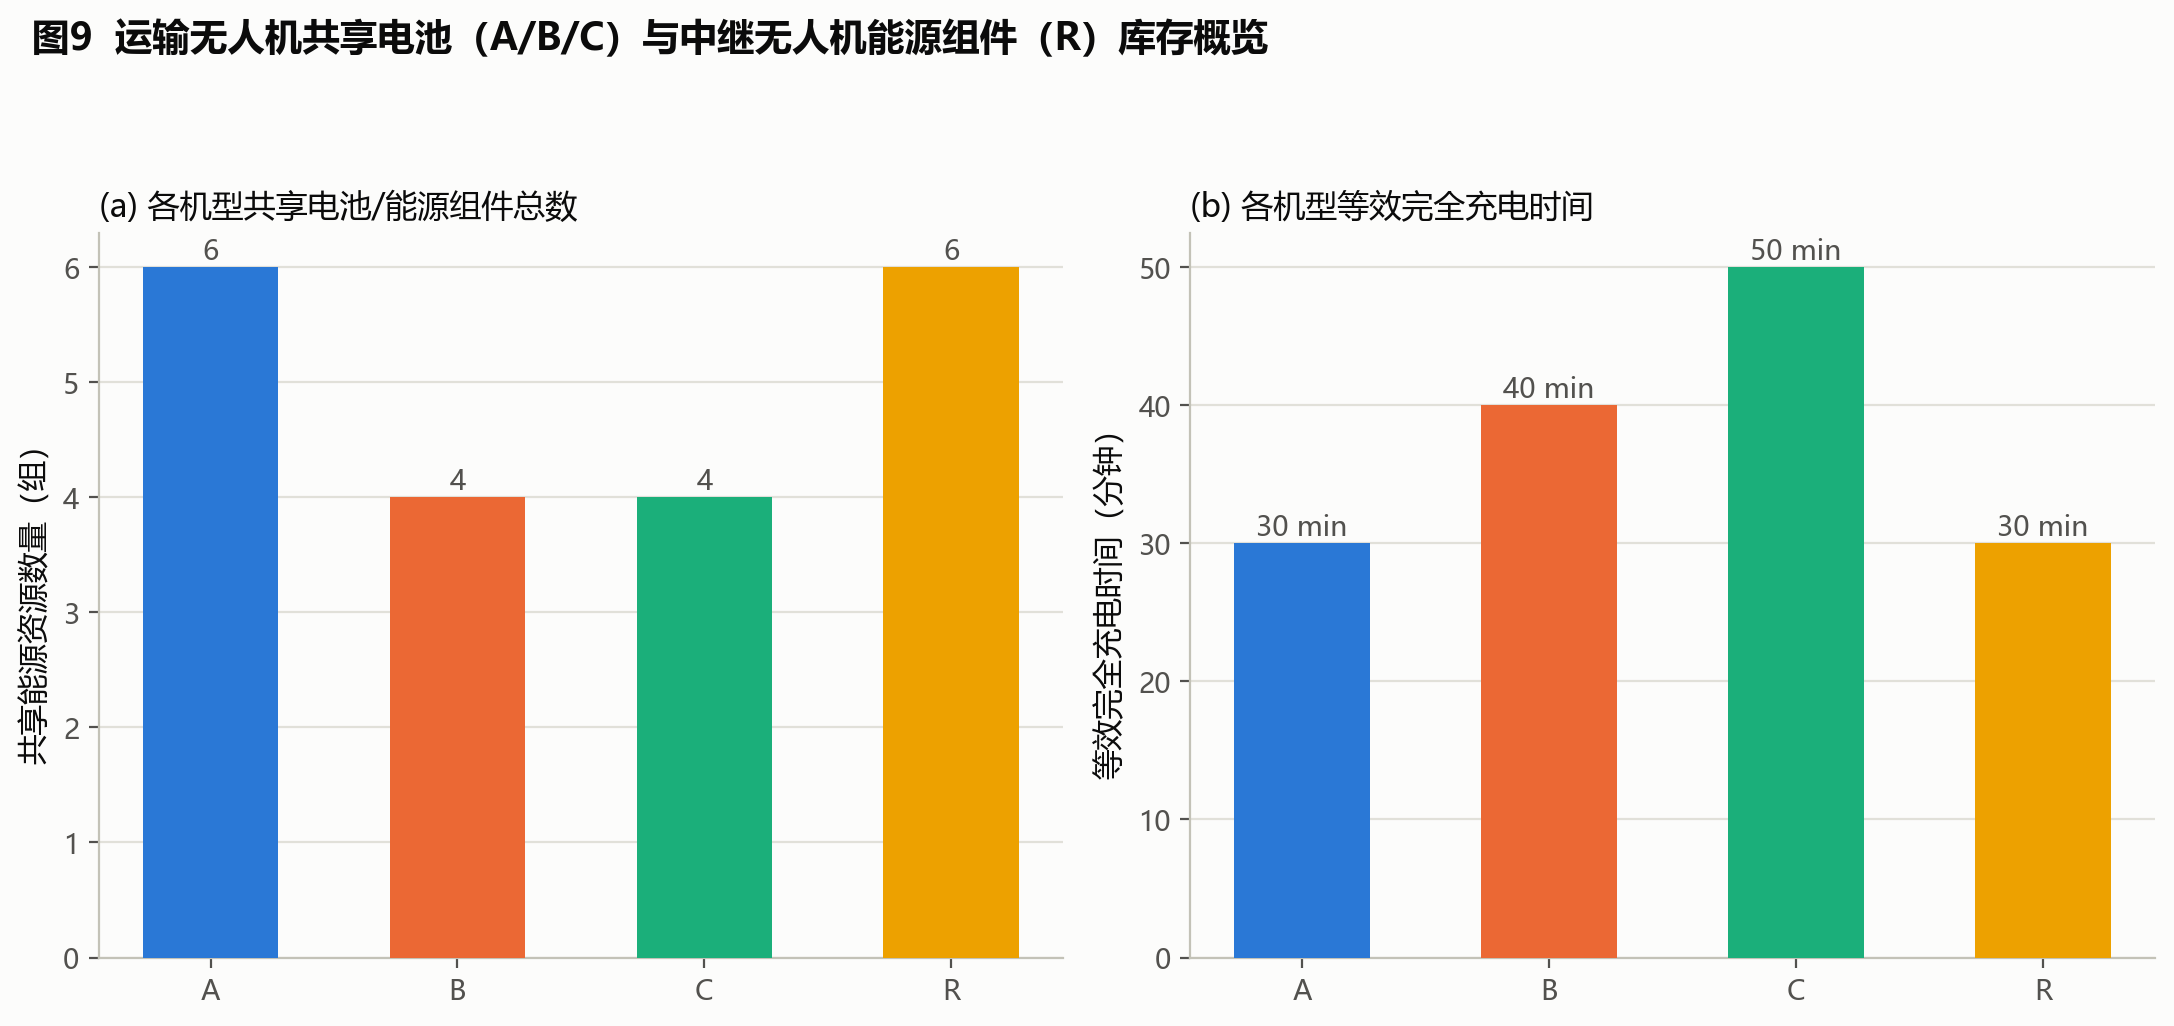
\includegraphics[width=0.48\textwidth]{figures/09_共享能源资源库存与充电时间.png}\label{fig:data_battery}}
\caption{运输无人机机型与共享电池参数}
\label{fig:data_drone_battery}
\end{figure}

\subsection{中继无人机与通信链路参数}

中继无人机（2 架）与可更换能源组件（6 个）构成独立的通信保障资源池。图~\ref{fig:data_relay} 给出中继无人机的巡航/爬升/下降/悬停功率与能源组件参数，其中悬停功率与通信附加功率共同决定中继服务能耗。图~\ref{fig:data_comm} 给出通信链路各主体的发射功率、天线增益、接收灵敏度等参数对比及链路预算，可见"运输—中继"接入链路与"中继—G01"回传链路的门限差异，是问题三双向链路可用性判定（取两方向较小门限）的数据基础。

\begin{figure}[htbp]
\centering
\subfloat[中继无人机参数]{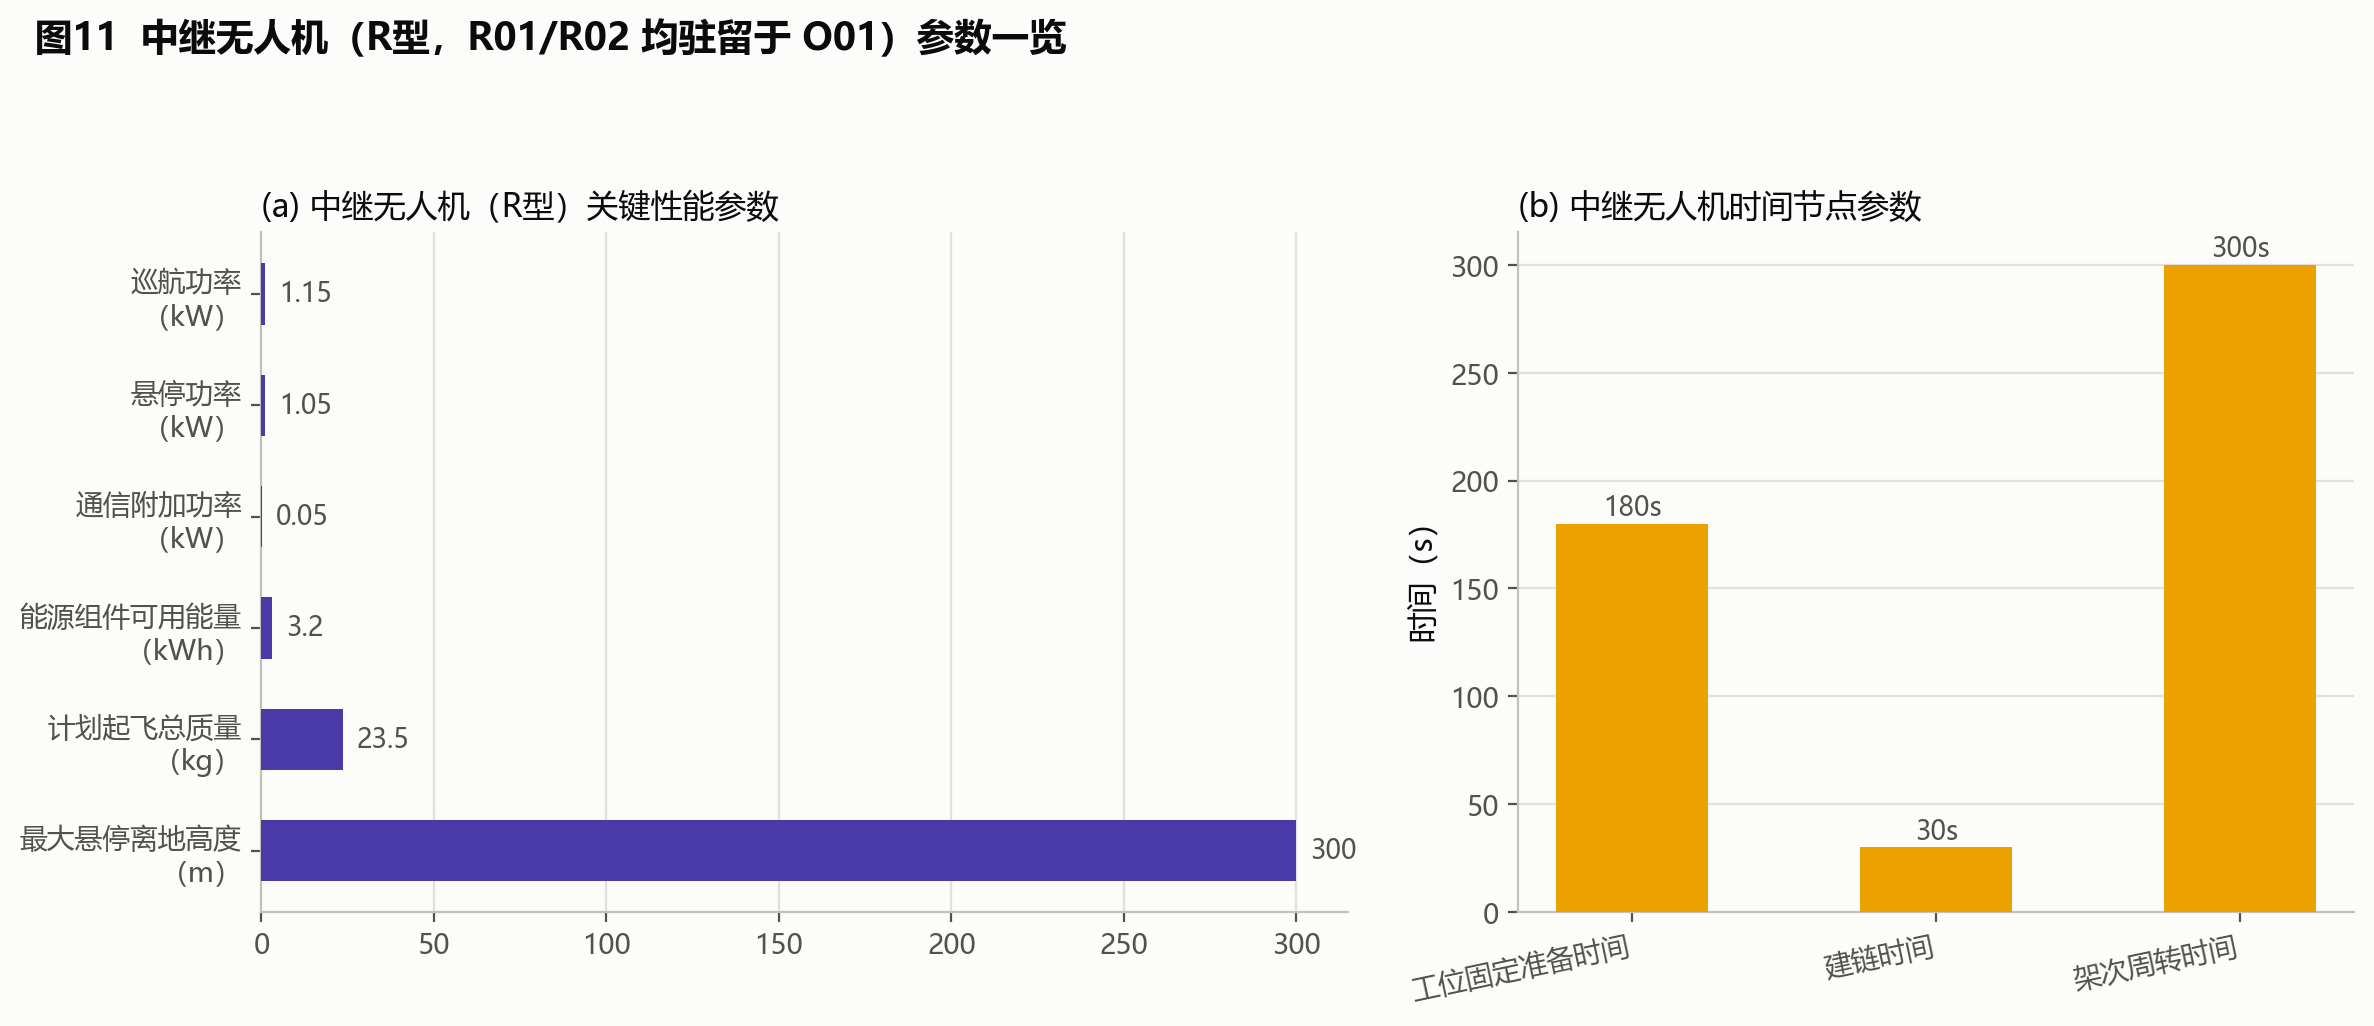
\includegraphics[width=0.48\textwidth]{figures/11_中继无人机参数一览.png}\label{fig:data_relay}}
\hfill
\subfloat[通信链路收发参数]{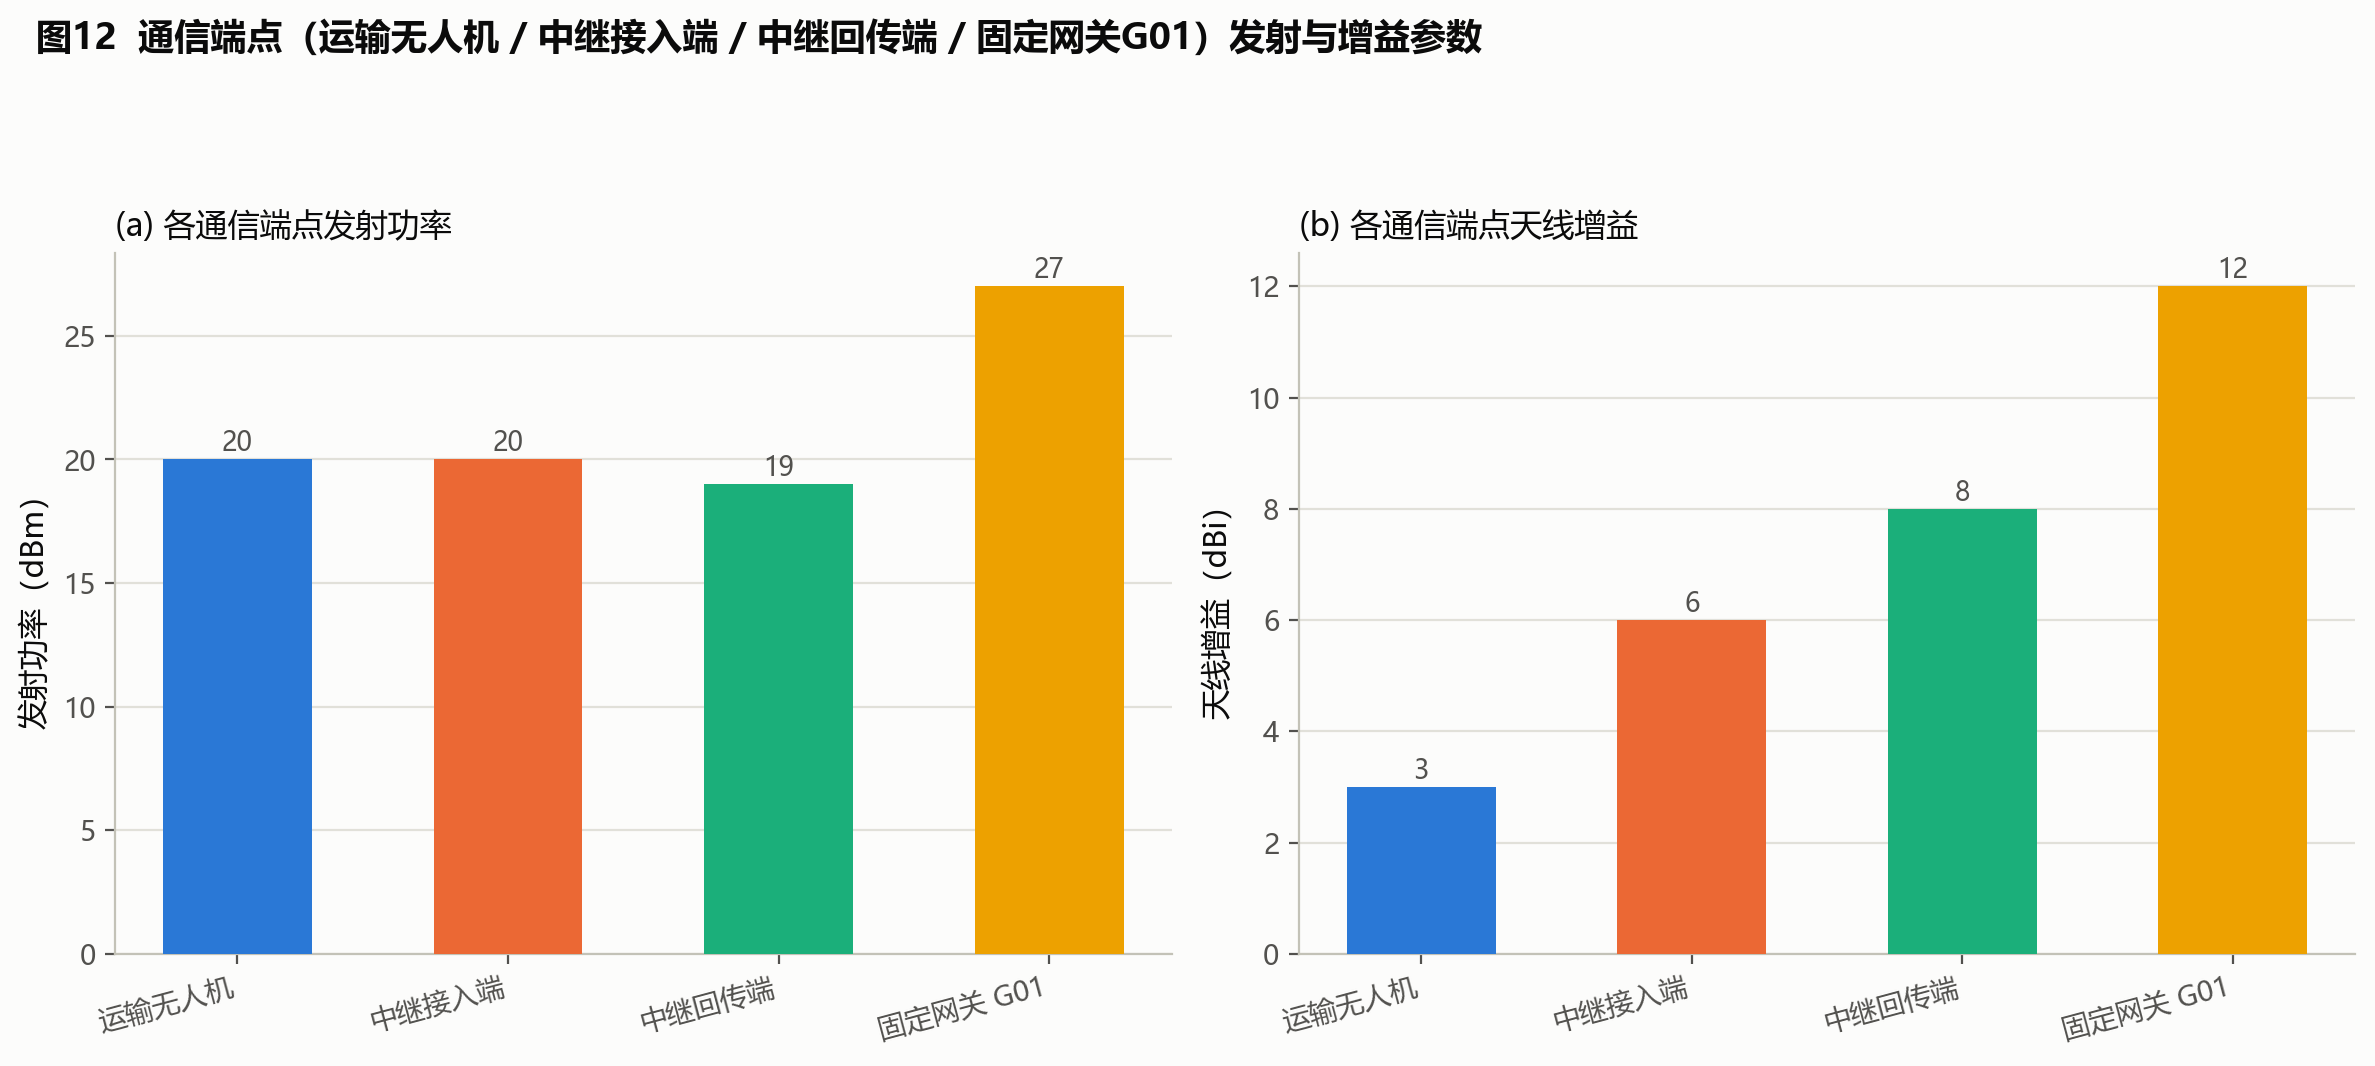
\includegraphics[width=0.48\textwidth]{figures/12_通信链路发射接收参数对比.png}\label{fig:data_comm}}
\caption{中继无人机与通信链路参数}
\label{fig:data_relay_comm}
\end{figure}

\begin{figure}[htbp]
\centering
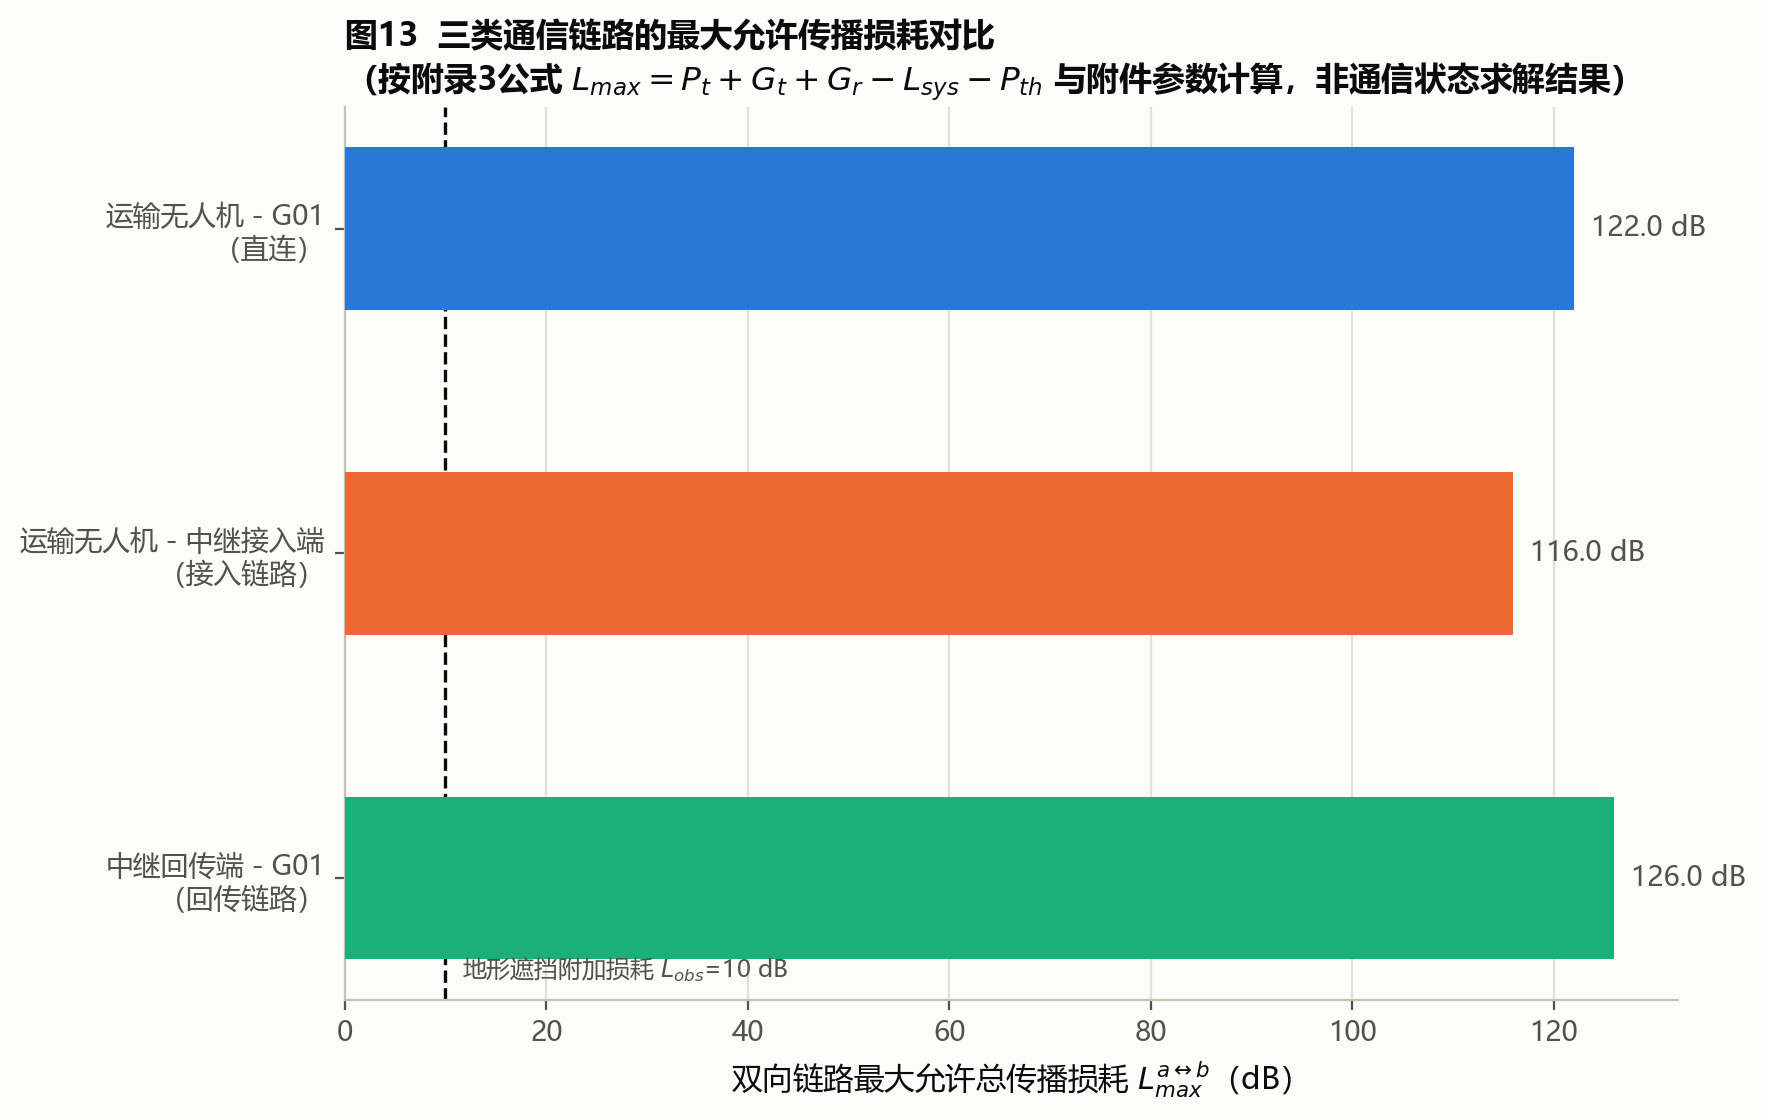
\includegraphics[width=0.6\textwidth]{figures/13_链路预算对比.png}
\caption{通信链路预算对比}
\label{fig:data_linkbudget}
\end{figure}

\subsection{数据预处理流程}

本文对原始数据做如下预处理，统一全文口径：(1) 节点经纬度经平面距离换算得到两节点水平距离，DEM 分辨率约 30\,m、CRS 为 EPSG:4326（与节点经纬度一致，无需重投影）；(2) 对任意节点对沿两节点水平直线对 DEM 逐像元采样，取路径最高地面高程用于计算计划巡航海拔（最高地面高程 $+50$\,m）；(3) 货箱清单按"首批保障、应急优先系数、单箱质量"降序排序，用于组批启发式与派单优先级；(4) 电池/能源组件按题设两阶段充电模型记录 SOC 与充电时段。上述预处理是问题一至问题四公共物理引擎的输入，保证了各问结果的可比性。
